



\chapter[Cryogenic Manipulation System]{Cryogenic Manipulation System}\label{chap-cryoMagnet}

This chapter is based on a Journal paper with Julien Leclerc, Benedict Isichei, and Aaron T. Becker.  The author's contribution was in the design of the heating elements interfacing the Manipulator and the robotic workspace, creating a camera mount for the system's sensory feedback, and working on the object tracking. 
Nathan Hui aided with editing the final version of the paper.


%%%%%%%%%%%%%%%%%%%%%%%%%%%%%%%%%%%%%%%%%%%%%%%%%%%%%%%%%%%%%%%%%%%%%%%%%%%%%%%%
\section{INTRODUCTION}
Magnetic actuation enables non-contact manipulation from a distance.  
This paper describes a magnetic manipulator, shown in Fig.~\ref{MagneticManipulatorPic}, that uses coils cooled by liquid nitrogen to reduce the size and power required to generate dynamic magnetic fields. 
Magnetic technologies have promise for several areas, including as actuation for minimally invasive surgery~\cite{Stereoaxis,nelson2010microrobots}.
Minimally invasive surgeries reduce patient recovery time, pain, and risks of infection~\cite{robinson2004minimally}. 
 These procedures are most often performed using a catheter, a tubular device that can access remote areas of the body through small incisions. 
  If all catheter actuation is applied at the proximal end, it is increasingly difficult to accurately control force and orientation of the distal tip as the length increases. 

% why magnetic actuation?  It already is being used!
 Magnetic actuation can be used to improve the effectiveness of minimally invasive surgeries. 
 The company Stereotaxis \cite{Stereoaxis} manufactures a magnetic system able to control the tip of a magnetic catheter and therefore increase the precision of the medical procedure. 
 The device uses two permanent magnets rotating around the workspace.
 \begin{figure}
	\includegraphics[width=\linewidth]{PictureManipulator.pdf}
	\caption{Picture of the magnetic manipulator while functioning. Inset shows view from the camera used to obtain position feedback of the robot.}
	\label{MagneticManipulatorPic}
\end{figure} 
 
 
 %As an example, coronary catheterization is a procedure consisting of inserting a catheter inside a blood vessel to access the coronary arteries. 
 Unfortunately, calcified fat deposits can build up inside arteries during the life of a person, a condition called atherosclerosis \cite{suri2010atherosclerosis}. 
 These deposits, called \emph{plaques}, may be detached by the friction between the catheter and the walls of the blood vessel and cause a stroke \cite{khatri2006ischemic,hamon2008periprocedural}.  
  \par
% Tetherless 
Tetherless magnetic robots could further decrease the invasiveness of procedures \cite{nelson2010microrobots}. 
The idea is to use external magnets to manipulate a small magnetic tool or capsule placed inside a patient. 
  The absence of tethers and the ability to navigate without touching the blood vessel walls \cite{kensicher2017towards} reduces the risk of plaque detachment. 
  A fast and accurate tracking method can enable precise control of the robot position during navigation. 
  However, permanent magnets are limited by their maximum rotational speed and acceleration and are therefore often unsuitable for fast dynamic control. 
 In contrast, electromagnets (EM) can generate magnetic fields with fast dynamics without moving parts. 
  Their magnetic field change rate is limited by either the power of the generator or the maximum voltage the magnet can sustain.
   \par
% About MRI
MRI scanners have EM and can be used as magnetic manipulators \cite{mathieu2006method, martel2007automatic, felfoul2016simultaneous}. 
 When a ferromagnetic piece (the robot) is placed inside this device, it becomes magnetized by the main magnetic field. 
  Because the main field is approximately uniform (less than 1 ppm of inhomogeneity \cite{wilson2002optimization}), it does not produce significant forces on the robot. 
  Instead, the MRI gradient coils can be used to produce a controlled force. 
 \par
 % Why MRI
The major advantage of using of MRI scanners for magnetic manipulation is that they are already widely available in hospitals and the robot's position can be tracked in real-time using the MR signal \cite{felfoul2009real, felfoul2016simultaneous}.
%the control is limited to three inputs as MRI scanners only have three sets of gradient coils. 
However, the large static magnetic field in an MRI permanently orients the magnetic field in the same direction, making torque control of robots impossible.
 The gradient coils can be used to generate forces on the robot.\par
% limitations on EMs
 Power consumption and heat dissipation are the primary limitations on EMs. 
 The current circulating inside a conductor produces Joule losses.
 Electromagnetic field strength is limited by its maximum power dissipation density. 
  More compact magnet designs can be achieved by reducing the amount of losses produced per unit of flux density. 
  If power consumption is not a concern, the maximum power dissipation density can also be increased.\par
 % discussion on ferromagnetic cores
Adding a ferromagnetic core to an EM is an effective way to increase the magnetic field and the forces produced without increasing the losses.
 Cores enable increasing the inductance value which in turn increases the total flux produced per ampere. 
 However, the use of a ferromagnetic core requires a closed bore geometry for the magnet. 
 This is often an issue for medical applications. 
  MRIs are designed with open bores on two opposite sides to accommodate the patient. 
 Additional openings could allow medical staff to access the patient during the procedure and decrease feelings of claustrophobia.\par    
 % Advantages of LN2
Using liquid nitrogen (LN2) is another way to decrease the amount of losses produced per unit of flux density. 
This method decreases the value of the electrical resistivity of copper and therefore allows more current to circulate inside the magnet for a given amount of losses. 
Cooling the EM to cryogenic temperatures offers another advantage: because the temperature of the coolant is low, the maximum safe temperature increase of the coil is larger. 
LN2 cooling therefore increases the maximum power dissipation density. 
LN2 is cheap (approximately 0.13 USD/Liter) and available in industrial quantities. 
It is non-toxic as gaseous nitrogen composes 78\% of the volume of our atmosphere. However, if large quantities of liquid nitrogen are evaporated, the level of oxygen in the room might decrease. An adapted ventilation system and a low oxygen alarm must be used to prevent anoxia. \par
% Outline
This paper presents the design and test of a magnetic manipulator cooled with LN2. 
A demonstration system is described in Section \ref{sec:System}.
The motivations and technical difficulties associated with this type of cooling are discussed in Section \ref{sec:CoolingWithLN2}.
A method to perform inverse magnetic calculations is then explained in Section \ref{sec:invMagnetics}.
 A robot trajectory controller is described in Section \ref{sec:TrajectoryControl}. 
 Next the system singularities are analyzed for 3-DOF control of a permanent magnet in Section \ref{sec:singularities}. 
  Experimental results are presented and analyzed in Section \ref{Experiment}. The paper concludes with lessons learned in this study.\par

%%%%%%%%%%%%%%%%%%%%%%%%%%%%%%%
\section{System Presentation}\label{sec:System}
The magnetic manipulator in Fig.~\ref{MagneticManipulatorPic} is designed to fit a human heart phantom. 
Detailed build instructions, a bill of materials, and CAD models are available\footnote{\href{https://github.com/RoboticSwarmControl/magnetic-manipulator-l2n-source}{github.com/RoboticSwarmControl/magnetic-manipulator-l2n-source}}.
The working volume is a sphere with radius 0.075 m. % $\SI{0.75}{\metre}$.
The system is composed of six copper coils arranged in a cubical shape (see Fig. \ref{CAD}). 
   Each coil is placed and held in an independent cryostat. 
 The cryostats contain the LN2 and were built using G10. 
 G10 is a fiberglass-epoxy composite able to withstand cryogenic temperatures. 
 Ordinary plastics become brittle at cryogenics temperatures, but G10 remains resilient. 
 G10 is also electrically nonconductive, an important feature to avoid induced currents.
 Induced currents generate a magnetic field that opposes variations in the applied field, making the system less responsive.
 Induced currents also generate heat.
%Induced currents generate a field that opposes the changing magnetic field.
\par
% induced currents oppose the changing magnetic field
% 
\begin{figure}
	%\includegraphics[width=\linewidth]{cadimage.png}
	\includegraphics[width=.7\linewidth]{Fig2exploded2sm.pdf}
	\caption{CAD model of the magnetic manipulator: (a) exploded view of three cryostats, (b) cross-section view.}
	\label{CAD}
\end{figure}
 Uninsulated G10 walls become cold and water present in air condenses and freezes on them. 
  This ice could interfere with objects in the workspace. 
  To prevent icing, the cryostat walls facing the workspace are insulated by a  10 mm thick layer of Styrofoam insulation.  %$\SI{10}{\milli\metre}$
Six acrylic plates (one for each internal face) containing a resistive heater and a  thermocouple temperature sensor cover the inner face of the insulation.
  The temperature of the internal walls surrounding the workspace are regulated using a real-time controller.
The evaporation rate  of LN2 is the product $\mathscr{L}\cdot P_o$,  where $\mathscr{L}$ is the latent heat of vaporization, equal to 200 kJ/kg for LN2 and $P_o$ is the power dissipated. The maximum power consumption of each coil of the system is 2 kW. 
At maximum power, 0.74 liters of LN2 evaporate per minute.
%  (2*10^3  J)/s*(60 s)/min*(1 kg)/(200*10^3  J)*1L/0.807kg = 0.74 L/min
 \par
%
\begin{figure*}[ht]
\centering
	\includegraphics[width=\linewidth]{FigureController.pdf}
	\caption{Block diagram of (a) the physical hardware and (b) the controller used for position control.
	\label{fig:Controller}	}
\end{figure*}
%
12 Kepco BOP 20-50 generators power the system. Each power supply can generate 20 A under 50 V. %$\SI{20}{\ampere}$ under $\SI{50}{\volt}$. 
 Each coil is powered by two of these supplies connected in series. Each coil can, therefore, receive a maximum of 20 A under 100 V. %$\SI{20}{\ampere}$ under $\SI{100}{\volt}$.
 Each set of power supplies is controlled via an analog input. 
 While the current inside an EM is directly proportional to the magnetic flux density produced, the voltage applied on an EM is proportional to the time derivative of the flux density. 
 It is therefore easier to control the produced magnetic field by controlling the current rather than the voltage on the EM. 
 The BOP power supplies can do this when controlled in current mode. 
 In this mode, the power supplies output a current proportional to an analog input.

An industrial controller IC-3173 from National Instrument is used for real-time computation, as shown in Fig.~\ref{fig:Controller}(a).
 A set of two Basler acA2040 cameras are attached at orthogonal faces of the magnetic manipulator. 
  These cameras are used to obtain robot position and orientation in real-time (100 Hz). 
   Two high precision NI 9263 analog modules are used to generate the analog signal controlling the power supplies.
   
   The laboratory is equipped with a low oxygen alarm (Honeywell BW Clip, approximately 140 USD).

\section{Cooling with Liquid Nitrogen}\label{sec:CoolingWithLN2}
\subsection{Motivations}
The voltage $U_l$ at the terminals of a resistive coil can be calculated using the following equation:
\begin{equation}
U_l=L\cdot\frac{\d I(t)}{\d t}+R(t)\cdot I(t),
\label{Ul}
\end{equation}
where $I$ is the current in the coil, $L$ is the coil inductance, and $R$ is the coil resistance.
Two components are present in this equation:
\begin{itemize}
\item The term $L\cdot \d I(t)/ \d t$ is related to the magnetic energy change rate. This term does not cause losses if a four quadrant power supply is used. This type of power supply has the ability to transfer stored magnetic energy back to the electrical network. It is desirable to maximize $L\cdot \d I(t)/ \d t$ because a high magnetic energy change rate generates a large force change rate, a desirable feature for robot control. 
\item The term $R(t)\cdot I(t)$ is associated with Joule losses. It is an undesirable term for two reasons. First, it causes the coil to heat and decreases the energy efficiency of the system. Secondly, power supplies are limited by their maximum voltage. The voltage across the coil is shared between the two terms of equation \ref{Ul}. If the term $R(t)\cdot~I(t)$ is increased, less voltage is available for the term $L\cdot \d I(t)/ \d t$. LN2 cooling allows reducing the value of $R(t)$ by 87\%;
\end{itemize}
%As shown in subsection \ref{Forward}, the force produced on a permanent magnet is proportional to the magnetic flux density. However, 
The magnetic flux $\Phi$ produced by a solenoid is proportional to its inductance as shown in 
\begin{equation}
\Phi (t)=L\cdot I(t).
\label{flux}
\end{equation}
 In \cite{kummer2010octomag}, the authors use a ferromagnetic core to increase the value of $L$ and therefore increase the amount of force generated. LN2 cooling is different and increases the generated field by increasing the value of $I(t)$.
  It is technically difficult to scale up magnetic manipulators \cite{kummer2010octomag}. 
  Air-cooled human-size manipulators would use comparitively large electromagnets to produce the magnetic field.
  This technical challenge could potentially be solved using LN2 cooling.  
  This type of cooling enables a significant decrease in the system price, size, mass and/or improve its energy efficiency. \par
  %
  This tendency is illustrated in Fig.~\ref{fig:ComparisonMagnetsDesigns} and Table \ref{DesignsCompare}, which compares the flux density magnitude produced by different EM designs along their revolution axis. 
 The comparison was computed using the magnetic modeling software Finite Elements Method Magnetics (FEMM \cite{meeker2010finite}).
 EM1 and EM3 correspond to the EM present in our experimental setup when respectively cooled with LN2 (EM1) and forced air (EM3).  
 The gain of flux density and magnetic gradient when cooling with LN2 is +435\% and is relatively equal to the gain in current (see Table \ref{CoolingComparison}). 
 EM2 and EM4 correspond to the same EM as 1 and 3 except that ferromagnetic cores were added to each. 
 The gain in flux density is small, approximately 10\%. 
 EM6 is a forced-air-cooled EM with a ferromagnetic core designed to generate the same magnetic field as EM1.  
  EM6 must be $2.5\times$ longer than EM1. 
  EM5 is the same as EM6 except that the ferromagnetic core was removed. 
  The relative gain in flux density obtained by adding a ferromagnetic core is larger for EM5 and EM6, suggesting that the gain is related to the aspect ratio of length/diameter of the coil.


%The amount of current that can circulate inside an EM is limited by its temperature. If the temperature become two high, the insulating wire will burn. Insulating varnishes are available in different classes depending on the maximum temperature tehy can withstand. For exemple, plain enamel is a class A insulator and can withstand a temperature of 378K. 
%The density of power released via Joule heating in a wire is equal to dP=rho.J2.dV with rho being the electric resistivity, J the current density and dV an infinitesimal volume element. The electrical resistivity of conducting materials varies a lot with temperature. At room temperature (300K) copper has an electrical resitivity of ??? ohm/m. When cooled at liquid nitrogen temperature (77K), it decreases to ??? ohm/m, approximately 7.7 times smaller. Accordinegely to eq. ?, if the electrical resistivity is divided by 100 then the current density must be multiplied by 10 to produce the same amount of losses. In other words, a copper EM working at a current I at room temperature can safely be operated at 10*I when cooled with LN2 as no more losses are produced. In practice, this value can be further increased because the coil will be able to tolerate more losses before damages appear. Indeed, the working temperature is lower and a larger temperature variation is therefore available before damages appear. In addition, the heat exchange coefficient is larger when cooling with LN2 compared to air.


%
\begin{table*}[ht]
\centering
%
\centering
\caption{Description of the electromagnet designs compared in Fig.~\ref{fig:ComparisonMagnetsDesigns}.}
\label{DesignsCompare}
\scalebox{0.8}{
\begin{tabular}{@{}lcccccc@{}}

\toprule
Electromagnet ID                    & 1               & 2               & 3          & 4          & 5  & 6        \\ \midrule
%Internal radius  $R_i$        & 90 mm          & 90 mm          & 90 mm     & 90 mm     & 90 mm & 90 mm    \\
External radius $R_e$         & 110 mm          & 110 mm          & 110 mm     & 110 mm     & 110 mm & 110 mm    \\
Coil width  $T_r$        & 20 mm          & 20 mm          & 20 mm     & 20 mm     & 20 mm & 20 mm    \\
Coil length  $T_z$                   & 20 mm           & 20 mm           & 20 mm      & 20 mm      & 50 mm & 50 mm     \\
Number of turns            & 795             & 795             & 795        & 795        & 1987 & 1987      \\
Copper wire                & AWG 22          & AWG 22          & AWG 22     & AWG 22     & AWG 22  & AWG 22    \\
Core                       & Air             & Hyperco-50      & Air        & Hyperco-50 & Air & Hyperco-50\\
Cooling method             & LN2 & LN2 & Forced air & Forced air & Forced air & Forced air \\
Max. cont. current & 7.5 A           & 7.5 A           & 1.4 A      & 1.4 A      & 1.4 A & 1.4 A \\
Schematic & \includegraphics[height=1.5cm]{Coil1Cold.pdf}   %TODO: add "LN2" text in the image
& \includegraphics[height=1.5cm]{Coil2Cold.pdf} 
& \includegraphics[height=1.5cm]{Coil3.jpg} 
& \includegraphics[height=1.5cm]{Coil4.jpg} 
& \includegraphics[height=1.5cm]{Coil5.jpg} 
& \includegraphics[height=1.5cm]{Coil6.jpg} 
\\\bottomrule
\end{tabular}}
% 
\end{table*}

%
\begin{figure}
\centering
	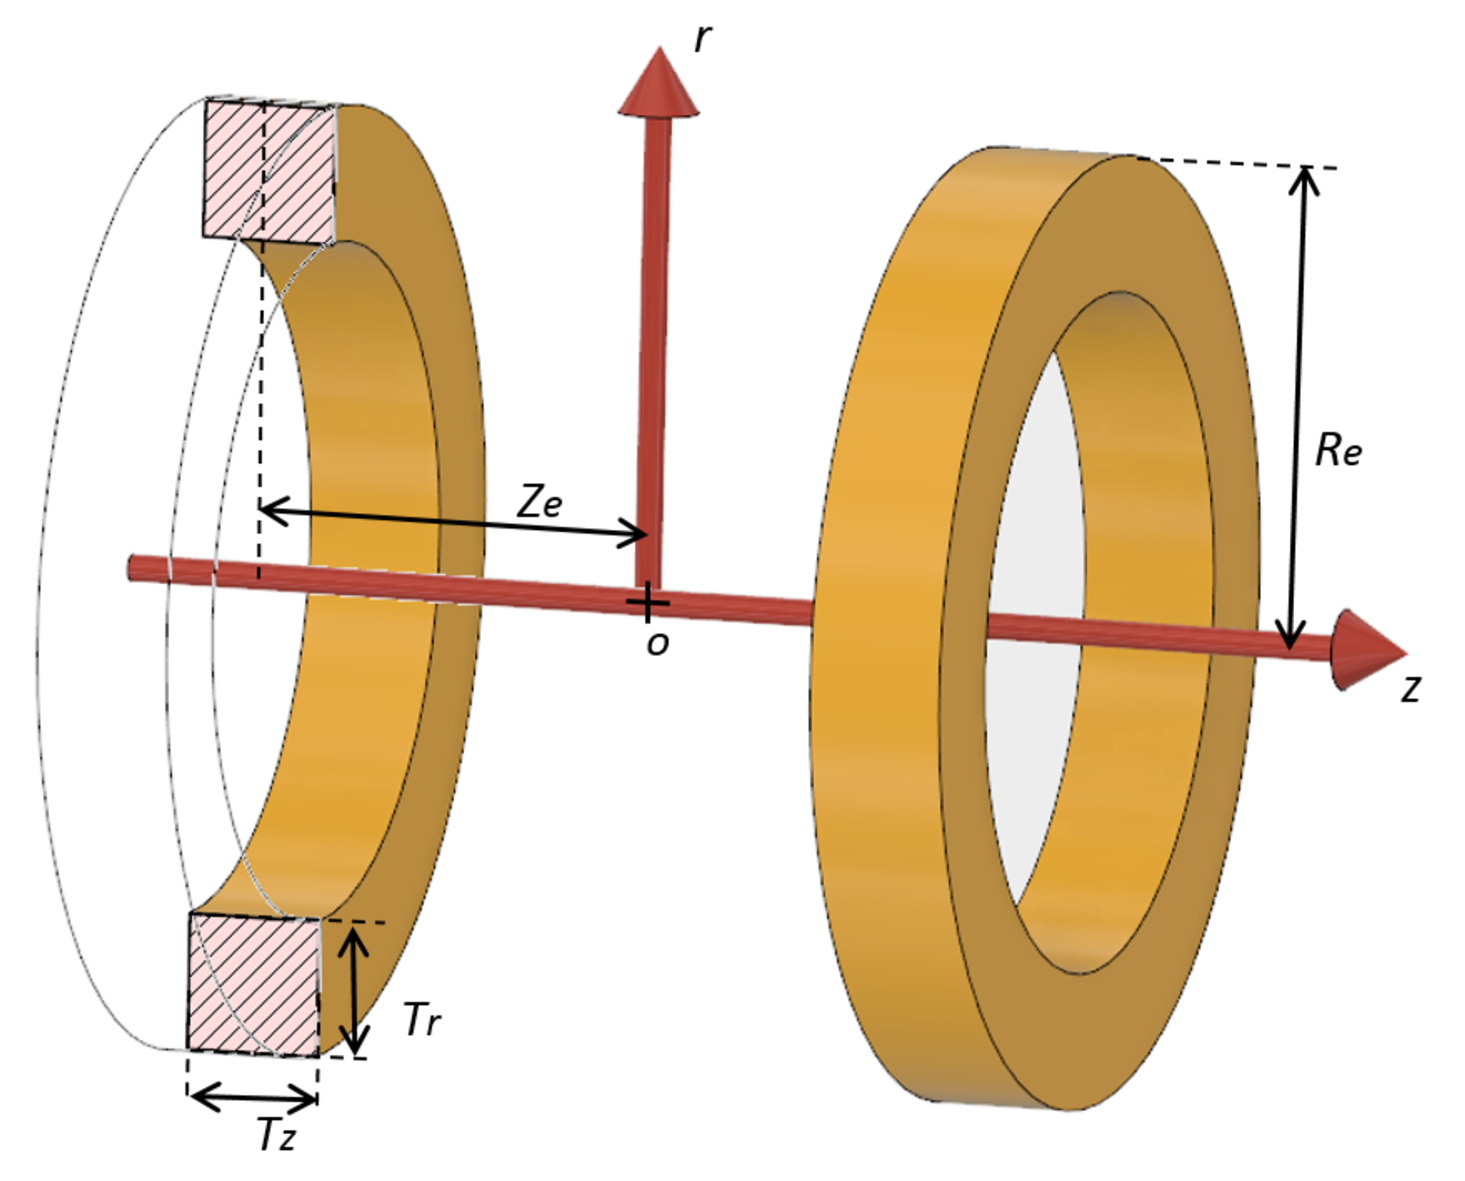
\includegraphics[width=0.5\linewidth]{3dView.eps}
	\caption{3D representation of a dual-coil collinear EM assembly.}
	\label{fig:3dView}
	\end{figure}


\begin{figure}
\includegraphics[width=\linewidth]{ComparisonMagnetsDesigns.pdf}
	\caption{ Maximum sustainable magnetic flux density  by different EM designs. Magnet specifications are given in Table \ref{DesignsCompare}.
	\label{fig:ComparisonMagnetsDesigns}}
\end{figure}

\subsection{Scaling Law}

This section uses analytical equations to derive the gradient produced by two concentric electromagnets on their revolution axis (see Fig. \ref{fig:3dView}). The electromagnets have an external radius $R_e$. They have a rectangular $T_z \times T_r$ cross-section. The filling factor $F_{\textrm{Fill}} $ is assumed to be equal to 0.7. LN2 cooled magnets have an additional insulation that has a thickness $T_{\textrm{insul}}$ which reduces the internal bore diameter $D_b$.

\begin{table}[]
\centering
\caption{Comparison between EM properties at room temperature (300K) and at LN2 temperature (77K).}
\label{CoolingComparison}
\begin{tabular}{@{}cccc@{}}
\toprule
 & 300K & 77K & Difference \\ \midrule
Copper electrical resistivity & 1.68E-8 $\Omega\cdot$m & 2.15E-9 $\Omega\cdot$m & -87\% \\ 
Coil electrical resistance & 27.3 $\Omega$ & 3.5 $\Omega$ & -87\% \\ 
Max continuous current & 1.4 A & 7.5 A & +435\% \\ 
Max cont. current density & 4.3 A/mm$^2$ & 23 A/mm$^2$ & +435\% \\ 
\bottomrule
\end{tabular}
\end{table}

The flux density $B_u$ produced by a single current loop can be calculated on its revolution axis using the Biot-Savart law:
%
\begin{equation}
B_{u}(R_u,Z_u)={\frac{\mu _0\cdot I_{u}}{2}}\cdot\left ( {\frac{R_{u}^2}{R_{u}^2+Z_u^2}} \right )^{\frac{3}{2}},
\label{bloop}
\end{equation}
%
where $R_u$ is the radius of the loop and $Z_u$ is the distance along the axis between the calculation point and the center of the loop.
The axial flux density created by a single finite EM is obtained by integrating this equation over the EM cross section:
%
\begin{align}
&\scalebox{.88}{$
B_e(R_e,Z_e) =
{\frac{J \mu _0   F_{\textrm{Fill}} }{2}} \int_{Z_e-T_z/2}^{Z_e+T_z/2} \int_{R_e-T_r}^{R_e} \left ( {\frac{R_{u}^2}{R_{u}^2+Z_u^2}} \right )^{\frac{3}{2}} \d R_u  \d Z_u 
$} \\
 &~~\scalebox{.7}{$=
  \frac{J \mu _0   F_{\textrm{Fill}}}{8}\left((T_z+2 Z_e) \left(\sqrt{4 R_e^2+(T_z+2 Z_e)^2}-\sqrt{4 (R_e-T_r)^2+(T_z+2 Z_e)^2}\right) \right. 
  $}  \nonumber \\
  & \qquad ~~~ \scalebox{.7}{$\left.+(T_z-2 Z_e) \left(\sqrt{4 R_e^2+(T_z-2 Z_e)^2}-\sqrt{4 (R_e-T_r)^2+(T_z-2 Z_e)^2}\right)\right)$} \nonumber,
\label{Be}
\end{align}
%
where $R_e$ is the external radius of the coil, $Z_e$ is the distance along the axis between the calculation point and the center of the coil, and $J$ is the current density inside the copper wire.
 The quantity $J\cdot F_{\textrm{Fill}} $ is the current density averaged over the winding $T_z \times T_r$ cross section.
  The magnetic gradient $G_e$ is calculated by the derivative of this equation with respect to $Z_e$:
\begin{equation}
G_e=\frac{\d B_e}{\d Z_e}.
\label{Ge}
\end{equation}

The total power $P_e$ dissipated inside the EM can be computed with:
%
\begin{equation}
P_e=\iiint_V F_{\textrm{Fill}}  \cdot \rho\cdot J^2 \,\d v, 
\label{Pe}
\end{equation}
%
over the volume $V$:
\begin{equation}
\scalebox{.9}{$V=\pi\ \left ( 2R_e \left ( R_e- T_{\textrm{insul}} -D_b \right ) -\left ( R_e-T_{\textrm{insul}}-D_b \right )^2\right ).$}
\label{V70cm}
\end{equation}
%
These equations were implemented in {\sc Matlab} with $T_z = T_r$. The function \texttt{fminsearch} was used to inverse this equation and find the value of $T_z$ that produces the desired gradient $G_e$ for a given $R_e$ and $Z_e$.

Fig. \ref{fig:ScalingLaw} presents simulation results obtained using equations \ref{bloop} to \ref{Pe}. Plot \emph{(a)} graphs the EM winding volume as a function of its external diameter. The red curves correspond to magnetic assemblies able to produce a gradient strength of 20 mT/m at the system center, while the blue curves correspond to magnetic assemblies  able to produce a gradient strength of 45 mT/m at the system center.. The value of $T_z$ and therefore the volume of the winding changes along these curves to produce the desired gradient strength.

Black curves have been added to locate the functioning points for a human-size system. They represent systems that have a 0.7 m bore diameter $D_b$ (similar to the bore diameters of MRI scanners). Dashed lines are plotted for an air cooled magnet while solid lines are for EM cooled with LN2.



To summarize, colored curved show systems that are able to produce a given gradient (20 mT/m for red curves and 45 mT/m for blue curves). 
 The value of $D_b$ is changing along these curves. Black curves represent systems that have $D_b$ values of 0.7 m. 
 The produced gradient strength is changing along these curves. 
  The intersections of the black and colored curves represent functioning points of systems able to produce a given gradient strength with a $D_b$ value of 0.7 m.
Plot \emph{(b)} in Fig.~\ref{fig:ScalingLaw} is similar to plot \emph{(a)} except that the results are presented in terms of power consumption. These data were obtained from the results presented in plot \emph{(a)} and calculated using eq. \ref{Pe}.

Results show that the windings of LN2 cooled systems are always smaller than air cooled windings. They also always use less power. A human-size system producing 45 mT/m would require EMs with a volume of 0.0117 m$^3$ and 0.0585 m$^3$ for LN2 and air-cooled EM respectively. Their power consumptions are respectively 17.2 kW and 8.56 kW. The use of LN2 therefore allows a reduction of 80\% of the winding volume and a decrease of 50\% of the power consumption.




\begin{figure}
	\centering
	\begin{overpic}[width=0.45\columnwidth]{ScalingLaw.eps}
	\end{overpic}
	\caption{Plot of the winding volume (a) and power consumption (b) of air-cooled (300K) and LN2-cooled (77K) EMs.}
	\label{fig:ScalingLaw}
\end{figure}



\section{Inverse Magnetics}\label{sec:invMagnetics}
This section analyzes 3D manipulation of a single robot having a magnetization $\mathbf{m}$. The magnetic manipulator is composed of six EM controlled by independent current sources. The total magnetic field is the sum of the field produced by each coil.
 This section calculates the coil current values to produce the desired force and torque on the robot or the desired force and magnetic field orientation.

\subsection{Forward problem} \label{Forward}
%To simplify the analysis, the forward problem will first be solved, i.e. from the current values, the force and flux density will be calculated.
To simplify analysis, we first solve the \emph{forward problem} which computes the force and flux density or force and torque using the coil currents. 

The system has six EMs, numerated from 1 to 6.
The magnetic flux density $B_{k(\mathbf{P})}$ produced by EM number $k$ at location $\mathbf{P}$ can be calculated using 
%
\begin{equation}
\mathbf{B}_{k(\mathbf{P})}=\begin{bmatrix}
B_{kx}
\\
B_{ky} 
\\ 
B_{kz}
\end{bmatrix}=\mathbf{\widetilde{B}}_{k(\mathbf{P})}\cdot I_k=
\begin{bmatrix}
{\widetilde{B}}_{kx(\mathbf{P})}
\\
{\widetilde{B}}_{ky(\mathbf{P})}
\\ 
{\widetilde{B}}_{kz(\mathbf{P})}

\end{bmatrix}\cdot I_k,
\label{FieldEq}
\end{equation}
%
 where $I_k$ is the current in the magnet and $\mathbf{B}_{k(\mathbf{P})}$ is a function that depends on the geometry of the system and the position of the magnet. The function $\mathbf{B}_{k(\mathbf{P})}$ is computed assuming that the coils are equivalent to current loops. The flux density produced by a current loop is calculated using the semi-analytical equations presented in \cite{simpson2001simple}.
The flux density produced by the complete system, $\mathbf{B}_{(\mathbf{P})}$, can be computed by summing the field produced by each magnet as
%
\begin{dmath}
\mathbf{B}_{(\mathbf{P})}= \scalebox{.8}{$\left(\mathbf{\widetilde{B}}_{1(\mathbf{P})}+\mathbf{\widetilde{B}}_{2(\mathbf{P})}+\mathbf{\widetilde{B}}_{3(\mathbf{P})}+\mathbf{\widetilde{B}}_{4(\mathbf{P})}+\mathbf{\widetilde{B}}_{5(\mathbf{P})}+\mathbf{\widetilde{B}}_{6(\mathbf{P})}\right )\mathbf{I} $},
\label{FieldTot}
\end{dmath}
%
 where $\mathbf{I}$ is a vector containing the current of each coil.

It is now necessary to define three new vectors:
%
\begin{align}
\mathbf{\widetilde{B}}_{x(\mathbf{P})}&= \scalebox{.85}{$\setlength\arraycolsep{2pt} \begin{bmatrix}
\widetilde{B}_{1x(\mathbf{P})} & \widetilde{B}_{2x(\mathbf{P})} & \widetilde{B}_{3x(\mathbf{P})} & \widetilde{B}_{4x(\mathbf{P})} & \widetilde{B}_{5x(\mathbf{P})} & \widetilde{B}_{6x(\mathbf{P})}
\end{bmatrix}$},
\label{Gx} \\
%
\mathbf{\widetilde{B}}_{y(\mathbf{P})}&= \scalebox{.85}{$\setlength\arraycolsep{2pt}
\begin{bmatrix}
\widetilde{B}_{1y(\mathbf{P})} & \widetilde{B}_{2y(\mathbf{P})} & \widetilde{B}_{3y(\mathbf{P})} & \widetilde{B}_{4y(\mathbf{P})} & \widetilde{B}_{5y(\mathbf{P})} & \widetilde{B}_{6y(\mathbf{P})}
\end{bmatrix}$}, \textrm{ and}
\label{Gy} \\
%
\mathbf{\widetilde{B}}_{z(\mathbf{P})}&= \scalebox{.85}{$\setlength\arraycolsep{2pt} \begin{bmatrix}
\widetilde{B}_{1z(\mathbf{P})} & \widetilde{B}_{2z(\mathbf{P})} & \widetilde{B}_{3z(\mathbf{P})} & \widetilde{B}_{4z(\mathbf{P})} & \widetilde{B}_{5z(\mathbf{P})} & \widetilde{B}_{6z(\mathbf{P})}
\end{bmatrix}$}.
\label{Gz}
\end{align}
%
Equation \ref{FieldTot} can be re-written as
\begin{equation}
\mathbf{B}_{(\mathbf{P})}=\begin{bmatrix}
\mathbf{\widetilde{B}}_{x(\mathbf{P})}
\\
\mathbf{\widetilde{B}}_{y(\mathbf{P})}
\\ 
\mathbf{\widetilde{B}}_{z(\mathbf{P})}
\end{bmatrix}\cdot\mathbf{I}.
\end{equation}
%
The force $\mathbf{F}$ is calculated with:
%
\begin{equation}
\mathbf{F}=\begin{bmatrix}
F_{x(\mathbf{P})}
\\ 
F_{y(\mathbf{P})}
\\ 
F_{z(\mathbf{P})}
\end{bmatrix}
=\mathbf{\nabla}\cdot\left ( \mathbf{m}\cdot\mathbf{B}_{(\mathbf{P})} \right ),
\label{Force}
\end{equation}
%
which can be re-written as:
%
\begin{equation}
\boldsymbol{F}=\begin{bmatrix}
m_x\cdot\frac{{\partial {\mathbf{\widetilde{B}}}_{x(\mathbf{P})}}}{\partial x}+m_y\cdot\frac{{\partial {\mathbf{\widetilde{B}}}_{y(\mathbf{P})}}}{\partial x}+m_z\cdot\frac{{\partial {\mathbf{\widetilde{B}}}_{z(\mathbf{P})}}}{\partial x}
\\ 
m_x\cdot\frac{{\partial {\mathbf{\widetilde{B}}}_{x(\mathbf{P})}}}{\partial y}+m_y\cdot\frac{{\partial {\mathbf{\widetilde{B}}}_{y(\mathbf{P})}}}{\partial y}+m_z\cdot\frac{{\partial {\mathbf{\widetilde{B}}}_{z(\mathbf{P})}}}{\partial y}
\\ 
m_x\cdot\frac{{\partial {\mathbf{\widetilde{B}}}_{x(\mathbf{P})}}}{\partial z}+m_y\cdot\frac{{\partial {\mathbf{\widetilde{B}}}_{y(\mathbf{P})}}}{\partial z}+m_z\cdot\frac{{\partial {\mathbf{\widetilde{B}}}_{z(\mathbf{P})}}}{\partial z}
\end{bmatrix}\cdot\mathbf{I}.
\end{equation}
%
The torque $\mathbf{T}$ is calculated with:
%
\begin{equation}
\mathbf{T}=\begin{bmatrix}
T_{x(\mathbf{P})}
\\ 
T_{y(\mathbf{P})}
\\ 
T_{z(\mathbf{P})}
\end{bmatrix}
=\mathbf{m}\times\mathbf{B},
\label{Torque}
\end{equation}
%
which can be re-written as
%
\begin{equation}
\mathbf{T}=\begin{bmatrix}
m_y\cdot \mathbf{\widetilde{B}}_{z(\mathbf{P})}-m_z\cdot \mathbf{\widetilde{B}}_{y(\mathbf{P})}
\\
m_z\cdot \mathbf{\widetilde{B}}_{x(\mathbf{P})}-m_x\cdot \mathbf{\widetilde{B}}_{z(\mathbf{P})}
\\ 
m_x\cdot \mathbf{\widetilde{B}}_{y(\mathbf{P})}-m_y\cdot \mathbf{\widetilde{B}}_{x(\mathbf{P})}
\end{bmatrix}\cdot \mathbf{I}.
\label{TorqueMatrix}
\end{equation}

\subsection{Inverse problem}
Two inverse methods are studied. The first one aims at controlling the flux density and the force applied on the robot using the actuation matrix $\mathbf{A_0}$:
%
\begin{equation}
\mathbf{A_0}=\begin{bmatrix}
\mathbf{\widetilde{B}}_{x(\mathbf{P})}
\\
\mathbf{\widetilde{B}}_{y(\mathbf{P})}
\\ 
\mathbf{\widetilde{B}}_{z(\mathbf{P})}
\\ 
m_x\cdot\frac{{\partial {\mathbf{\widetilde{B}}}_{x(\mathbf{P})}}}{\partial x}+m_y\cdot\frac{{\partial {\mathbf{\widetilde{B}}}_{y(\mathbf{P})}}}{\partial x}+m_z\cdot\frac{{\partial {\mathbf{\widetilde{B}}}_{z(\mathbf{P})}}}{\partial x}
\\ 
m_x\cdot\frac{{\partial {\mathbf{\widetilde{B}}}_{x(\mathbf{P})}}}{\partial y}+m_y\cdot\frac{{\partial {\mathbf{\widetilde{B}}}_{y(\mathbf{P})}}}{\partial y}+m_z\cdot\frac{{\partial {\mathbf{\widetilde{B}}}_{z(\mathbf{P})}}}{\partial y}
\\ 
m_x\cdot\frac{{\partial {\mathbf{\widetilde{B}}}_{x(\mathbf{P})}}}{\partial z}+m_y\cdot\frac{{\partial {\mathbf{\widetilde{B}}}_{y(\mathbf{P})}}}{\partial z}+m_z\cdot\frac{{\partial {\mathbf{\widetilde{B}}}_{z(\mathbf{P})}}}{\partial z}
\end{bmatrix}.
\end{equation}
%
The force and flux density are equal to:
\begin{equation}
\label{FullEq}
\begin{bmatrix}
\mathbf{B}
\\ 
\mathbf{F}
\end{bmatrix}=\mathbf{A_0}\cdot\mathbf{I}.
\end{equation}
$\mathbf{A_0}$ is a square matrix and can be inverted provided that it is not singular. The current $\mathbf{I}$ is calculated with:
%
\begin{equation}
\mathbf{I}=\mathbf{A_0}^{-1}\cdot\begin{bmatrix}
\mathbf{B}
\\ 
\mathbf{F}
\end{bmatrix}.
\end{equation}
%
The second method controls the force and torque applied on the robot using the actuation matrix $\mathbf{A_1}$
%
\begin{equation}
\mathbf{A_1}=\begin{bmatrix}
m_y\cdot \mathbf{\widetilde{B}}_{z(\mathbf{P})}-m_z\cdot \mathbf{\widetilde{B}}_{y(\mathbf{P})}
\\
m_z\cdot \mathbf{\widetilde{B}}_{x(\mathbf{P})}-m_x\cdot \mathbf{\widetilde{B}}_{z(\mathbf{P})}
\\ 
m_x\cdot \mathbf{\widetilde{B}}_{y(\mathbf{P})}-m_y\cdot \mathbf{\widetilde{B}}_{x(\mathbf{P})}
\\
m_x\cdot\frac{{\partial {\mathbf{\widetilde{B}}}_{x(\mathbf{P})}}}{\partial x}+m_y\cdot\frac{{\partial {\mathbf{\widetilde{B}}}_{y(\mathbf{P})}}}{\partial x}+m_z\cdot\frac{{\partial {\mathbf{\widetilde{B}}}_{z(\mathbf{P})}}}{\partial x}
\\ 
m_x\cdot\frac{{\partial {\mathbf{\widetilde{B}}}_{x(\mathbf{P})}}}{\partial y}+m_y\cdot\frac{{\partial {\mathbf{\widetilde{B}}}_{y(\mathbf{P})}}}{\partial y}+m_z\cdot\frac{{\partial {\mathbf{\widetilde{B}}}_{z(\mathbf{P})}}}{\partial y}
\\ 
m_x\cdot\frac{{\partial {\mathbf{\widetilde{B}}}_{x(\mathbf{P})}}}{\partial z}+m_y\cdot\frac{{\partial {\mathbf{\widetilde{B}}}_{y(\mathbf{P})}}}{\partial z}+m_z\cdot\frac{{\partial {\mathbf{\widetilde{B}}}_{z(\mathbf{P})}}}{\partial z}
\end{bmatrix}.
\label{A1}
\end{equation}

The torque and force are equal to:

\begin{equation}
\label{FullEq2}
\begin{bmatrix}
\mathbf{T}
\\ 
\mathbf{F}
\end{bmatrix}=\mathbf{A_1}\cdot\mathbf{I}.
\end{equation}
$\mathbf{A_1}$ is a square matrix and can be inverted provided that it is not singular. The current $\mathbf{I}$ is calculated with:
\begin{equation}
\mathbf{I}=\mathbf{A_1}^{-1}\cdot\begin{bmatrix}
\mathbf{T}
\\ 
\mathbf{F}
\end{bmatrix}.
\label{FullEq3}
\end{equation}


\section{Trajectory control}\label{sec:TrajectoryControl}


Equation \ref{FullEq} shows that $\mathbf{F}$ is decoupled from $\mathbf{B}$ and $\mathbf{T}$. The control of $\mathbf{B}$ enables the control of the orientation of the robot. The robot can be assumed to be oriented along the magnetic field direction, as in~\cite{kummer2010octomag}. The magnitude of the flux density $|\mathbf{B}|$ is set to a constant value and the individual components are calculated to obtain the desired field orientation. Another alternative is to use eq. \ref{FullEq3} to control the torque directly.

The trajectory is controlled using the controller presented in Fig.~\ref{fig:Controller}(b). It uses a nested control structure. 
The inner PID control loop regulates velocity, which is limited by a saturation function to avoid excessive speeds and instabilities. 
The outer loop generates a velocity setpoint.\par

The trajectory is defined by the user as a set of of viapoints and the corresponding desired velocities $V_t$. The outer loop first searches for the point of the trajectory that is the closest to the robot position and determines $V_t$. An additional velocity component $V_s$ is added to this value to steer the robot toward the trajectory centerline.\par
  
When the calculated current is above the maximum value ($I_{\textrm{max}}$ is the maximum current the power supplies can generate) the vector $\mathbf{I}$ is scaled down so that the largest element of $\mathbf{I}$ is equal to $I_{\textrm{max}}$. 
This reduces the force and flux density values applied on the robot, but has the advantage of keeping the correct field and force orientation. 



\section{Singularities analysis for a 3-DOF robot} \label{sec:singularities}
%\begin{figure}
	%\begin{overpic}[width=\linewidth]{Condition.eps}
	%\put(32,86){\includegraphics[width=0.4cm]{TinyMag0.pdf}}
	%\put(83,86){\includegraphics[width=0.4cm]{TinyMag90.pdf}}
	%\put(32,41){\includegraphics[width=0.4cm]{TinyMagn45.pdf}}
	%\put(83,41){\includegraphics[width=0.4cm]{TinyMag45.pdf}}
	%\end{overpic}
	%\caption{Condition number of $\mathbf{A}$ at four robot angle $\theta$ values.}
	%\label{Condition}	
%\end{figure}

\begin{figure}
	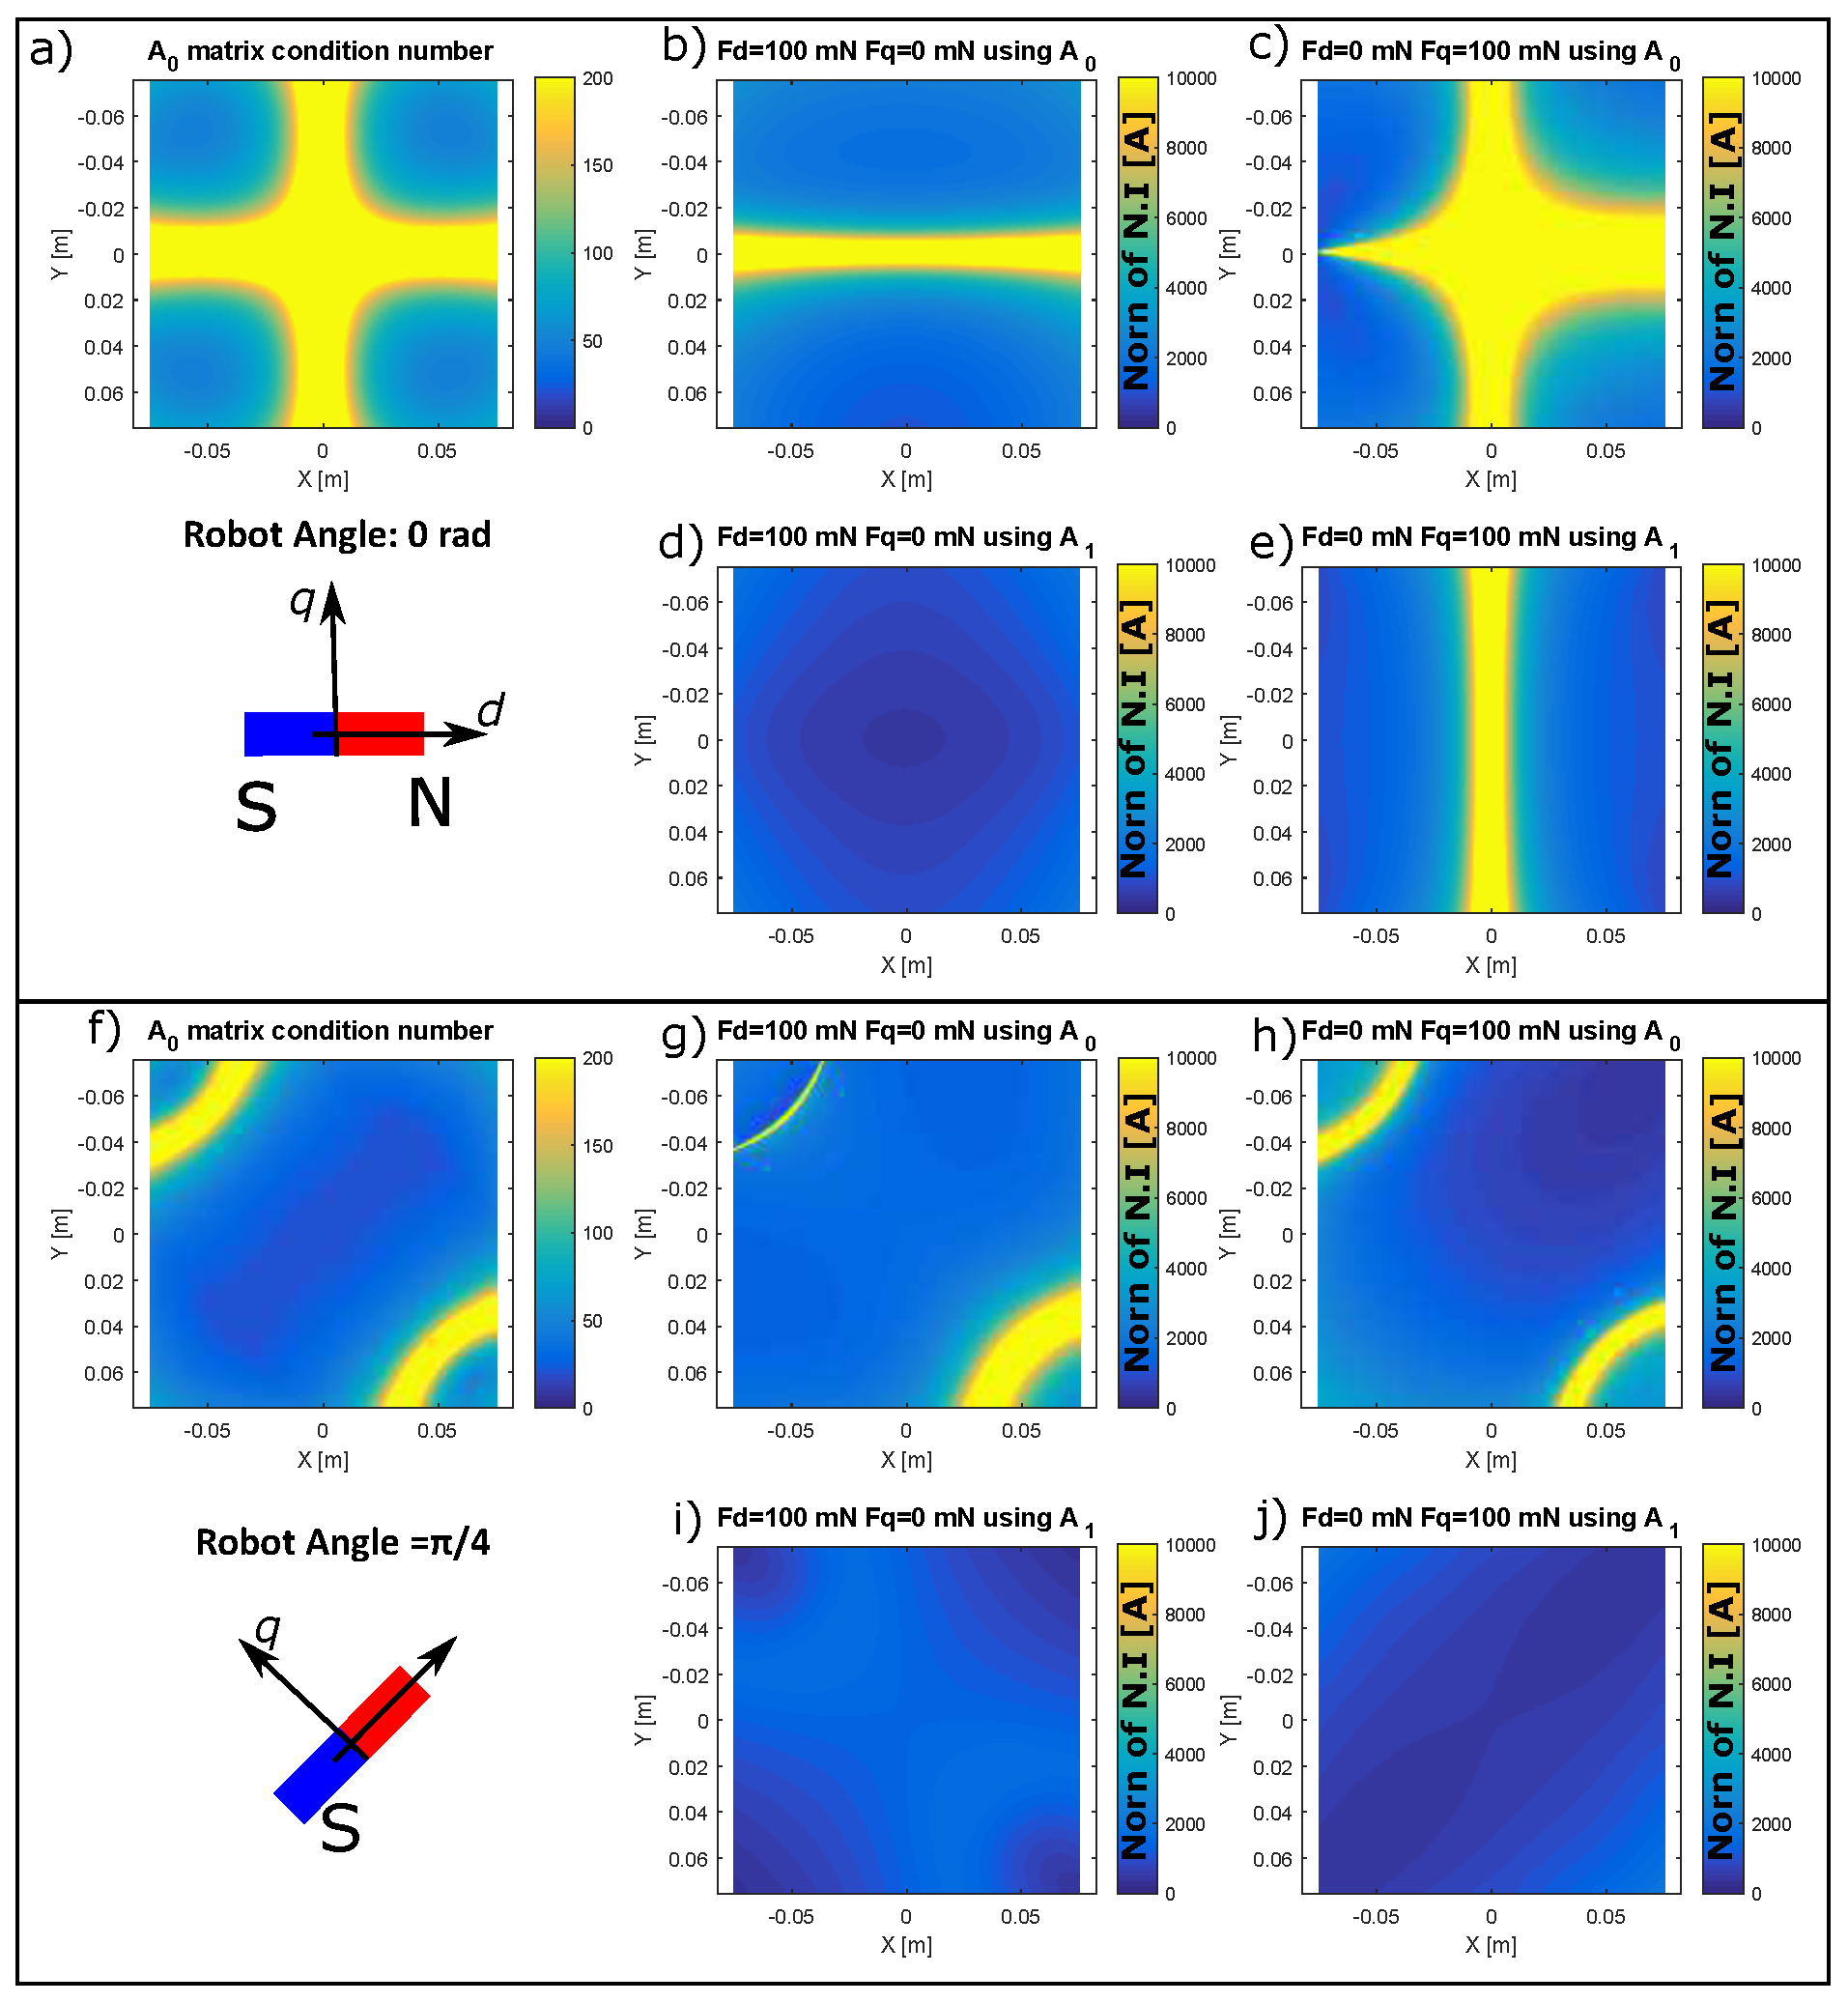
\includegraphics[width=\linewidth]{Conditioning3.eps}
	\caption{Map of the conditioning of the actuation matrix $\mathbf{A_0}$ for (a) $\theta=0$ and (f) $\theta=\pi/4$. 
	Map of the norm of the total current needed to produce a force of 100 mN along the $d$ axis (b, d, g and i) and along the $q$ axis (c, e, h and j).  }
	\label{condition}
\end{figure}


As explained in Section \ref{sec:TrajectoryControl}, the orientation of the robot can be controlled using two different methods. 
 The first one uses actuation matrix $\mathbf{A_0}$ and allows applying a desired flux density vector $\mathbf{B}$ and a force $\mathbf{F}$ to the robot. 
 The second uses actuation matrix $\mathbf{A_1}$ and allows applying a desired torque $\mathbf{T}$ and a force $\mathbf{F}$ to the robot.

When expressed in the manipulator coordinate system ($x,y,z$), $\mathbf{A_1}$ is square. However, the robot is symmetric around its revolution axis $d$ and therefore no torque can be applied on the $d$ axis. Defining a new coordinate system ($d,q,w$) allows removing one dimension from $\mathbf{A_1}$ (i.e. $\mathbf{A_1}$ has a size 5$\times$6 when expressed in the ($d,q,w$) coordinate system). The system is therefore underdetermined and the least square solution is calculated using 
 
\begin{equation}
\label{LS}
\mathbf{I}=\mathbf{A_1}^{T}\left ( \mathbf{A_1} \cdot \mathbf{A_1}^{T} \right )^{-1}\cdot \begin{bmatrix}
\mathbf{T}
\\ 
\mathbf{F}
\end{bmatrix}.
\end{equation}

The actuation matrices $\mathbf{A_0}$ and $\mathbf{A_1}$ are functions of the magnetic manipulator geometry and the robot pose. 

The effect of singularities was studied for a 2D--3DOF control. The magnet is horizontally placed on a flat surface corresponding to the $x$-$y$ plane. The robot is able to move along $x$ and $y$ and rotate around the $z$-axis.

A 4$\times$4 $\mathbf{A_0}$ and a 4$\times$3 $\mathbf{A_1}$ actuation matrices can be calculated for each robot position and angle. The map of the conditioning of the $\mathbf{A_0}$ matrix is shown in Fig.~\ref{condition}(a) and (f). On this figure is also presented the norm of the total current $N \cdot \mathbf{I}$ required to produce a force of 100 mN along the $d$-axis (central-column) and $q$-axis (right-column). Plots b, c, d and e are plotted for $\theta=0$ and plots g, h, i and j are plotted for $\theta=\pi/4$. Plots b, c, g and h were calculated using $\mathbf{A_0}$ and plots d, e, i and j were calculated using $\mathbf{A_1}$.

For $\theta=0$, $\mathbf{A_0}$ has two singularity lines on the $x$ and $y$ axis. For $\theta=\pi/4$ singularities take a rounded shape and are located on two opposite angles of the workspace. No solution is available when the matrix is singular. The singularities are situated on infinitely thin lines, but the system is ill-conditioned near the singularity lines. A large condition number produces a large magnitude for the $\mathbf{I}$ vector. The capabilities of the power supplies limit the maximum current and when the condition number becomes too large, the current saturates. This saturation decreases control authority over the robot in these regions.\par

The norm of the total current $N \cdot \mathbf{I}$ needed to produce a force of 100 mN along the $d$ and $q$ axis was calculated as a function of the robot position and angle. Plots b, c, e and f of Fig.~\ref{condition} present these results. When using the $\mathbf{A_0}$ matrix, there are areas where the current becomes larger than 10,000~A close to the singularities when the force is generated along the $d$ axis as well as when the force is generated along the $q$ axis. When using $\mathbf{A_1}$, these large current densities are present only when a force is generated along the $q$ axis. When the force is produced along the $d$ axis, the current always stays within relatively small values. This observation is valid for any robot orientation.

\section{Experimental Results}
\label{Experiment}
\begin{figure}
\includegraphics[width=\linewidth]{EllipseTrajectory.eps}
\vspace{-2em}
	\caption{Plot of the trajectory of the robot obtained experimentally. For this dataset, the robot completed the path ten times. The robot and the workspace are shown at right.}
	\label{Path}	
\end{figure}

\begin{figure}
	\includegraphics[width=\linewidth]{Waveform.eps}
	\caption{Voltage, current, and power used during robot navigation. The curves show 60 seconds of data, which correspond to the robot completing the trajectory in Fig.~\ref{Path} three times.}
	\label{waveform}
\end{figure}

The control of the velocity and orientation of a NdFeB permanent magnet in a 2D plane described in Section \ref{sec:TrajectoryControl} was implemented and tested using the $\mathbf{A_1}$ actuation matrix. As shown in Section \ref{sec:singularities} it is preferable to apply the force along the magnetization axis of the robot ($d$-axis). The program was therefore configured to orient the robot magnetization in the same direction as the applied force. This allows minimizing the value of the force applied along the $q$ axis and therefore improve stability by avoiding current saturations.
% As shown in Section \ref{sec:singularities} 
The permanent magnet was cylindrical, with a diameter of 2.5 mm and a length of 10 mm. 
It was encapsulated in a black shrink tube to facilitate computer vision tracking. 
The magnet was then attached horizontally on a Styrofoam disk having a diameter of 18 mm and a thickness of 6 mm. 
Pictures of the robot are shown in Fig.~\ref{Path}. 

A robot navigating inside fluid-filled cavities of the human body may be designed to have neutral buoyancy to reduce the amount of force needed. 
To simulate neutral buoyancy in this 2D control experiment, the magnet-Styrofoam assembly floated at the surface of a water-filled tank. The magnet was able to move freely in the $x$ and $y$ directions as well as rotate around the $z$ axis.\par
The method from Section \ref{sec:TrajectoryControl} was used with the $\mathbf{A_1}$ actuation matrix from \eqref{A1}.
 The trajectory was an ellipse having a major axis of 63 mm and a minor axis of 40 mm.

Test were performed with and without LN2 cooling. The trajectory obtained experimentally without LN2 is presented in Fig.~\ref{Path}. For these plots, the robot followed the trajectory ten times. Trajectories obtained with LN2 cooling are similar. The robot was stable during the navigation, but small deviation from the centerline were observed at several locations. 

The current and voltage applied on the $-x$ EM was recorded during one minute for both cooling methods. The instantaneous power was calculated from these data and the results are presented in Fig. \ref{waveform}. The average power used for the air cooled case is equal to 0.218 W whereas it is only equal to 0.037 W when magnets are cooled with LN2.  This decrease of average power consumption is enabled by the decrease of copper electrical resistivity when cooled at 77K and produces a decrease of the applied voltage as shown in  Fig.~\ref{waveform}(a).  The parameters of the controller were not changed between the tests, however, the peak power is increased when LN2 is added. This behavior could be explained by an increase of the current regulation dynamics performed by the power supply when the electrical resistance of the EM is decreased by the cooling. 

The power used was low because the floating robot required little force.
%The values of power obtained are low due to the fact that the force that needs to be applied on a floating robot to move it is very small. 
Applications that navigate against flow or perform surgery require larger forces and correspondingly more power.


 
% 
%The conclusion looks like a summary. It shouldn�t. You can focus on if
%your main hypotheses of the paper could be supported by the experiment
%etc., and other derivatives of the hypotheses.
%%%%%%%%%%%%%%%%%%%%%%%%%%%%%%%%%%%%%%%%%%%%%%%%%%%%%
\section{Conclusion and Future Works}
%%%%%%%%%%%%%%%%%%%%%%%%%%%%%%%%%%%%%%%%%%%%%%%%%%%%%
This paper presented a magnetic manipulator using EM cooled with LN2. 
Liquid nitrogen cooling allows increasing the current circulating inside an EM up to 435\%. 
This cooling enables reducing the size of the EM to produce a given magnetic field. 
The required electromagnets to achieve a given flux density are cheaper to build, and the complete system is more compact. 
%Air-core LN2-cooled EM can, unlike iron-core magnets, have an open bore. 
%This feature is necessary for medical applications where the magnetic system needs to be open on at least two opposite ends to accommodate the patient.
\par
%
A desktop-size prototype was built and tested. 
The robot, a cylindrical permanent magnet, was manipulated on a 2D plane. 
Three DOF were controlled: the orientation and the $x$ and $y$ positions.\par
%
The system was not designed to produce a uniform magnetic field. 
Instead, inverse magnetic calculations account for field non-uniformities.
The current inside each coil is computed to generate the desired force on the robot and produce the desired field orientation. 
 %The calculations include a function that computes the field produced by each coil in space. 
 %The coils are assumed to be equivalent to circular current loops.
 \par
 %
The system's matrix conditioning was analyzed. 
 The matrix is sometimes ill-conditioned, depending on the position and orientation of the robot. 
  Issues with ill conditioning can be avoided by controlling the torque directly and avoiding the production of forces along the axis perpendicular to the robot magnetization.
  \par
  %
More control inputs can be added to improve the controllability of the robot. 
A possibility is to use additional EM, as in \cite{kummer2010octomag} where eight EMs were used to control a five DOF robot, but using additional EMs makes the system more complicated and expensive to build.
 \par
 %
Future study will focus on the addition of a high-frequency component to the magnetic field to increase the controllability of the robot. 
  A permanent magnet could be encapsulated in a conductive shell such as copper. 
  If the robot is electrically conductive, the AC field would induce currents in it, and generate an additional torque as in an induction electric motor. 
  This AC magnetic field could also be used to control resonating magnetic actuators as in \cite{vollmers2008wireless}. 
  Finally, the controller could include a temperature management feature that calculates the heat dissipated in the windings and avoids overheating by preventively reducing power.
  %Mechanically resonating millirobots were successfully tested \cite{vollmers2008wireless,frutiger2008magmites}. 
%

